\documentclass[a4paper, pdftex, 14pt, oneside, titlepage, openany, onecolumn]{book}
\usepackage[spanish]{babel}
\usepackage[utf8]{inputenc}
\usepackage[T1]{fontenc}
\usepackage[pdftex]{graphicx}
\usepackage{makeidx} 
\usepackage{fancyhdr}
\usepackage{listings}
\usepackage{tikz}
\usepackage{setspace}
\newcommand{\HRule}{\rule{\linewidth}{0.5mm}}

\begin{document} 
\pagestyle{fancy}
\renewcommand\headrulewidth{0pt}
\setlength{\parskip}{16pt}
\onehalfspace
\lhead{}

\author{Yohan Graterol B.}
\title{NoSQL y MongoDB en Español}
\date{Dic 2013}

\begin{titlepage}
	\begin{center}
		
\includegraphics[scale=0.10]{img/mongodb}
		\HRule \\[0.4cm]
		{ \huge \bfseries NoSQL y MongoDB en Español \\[0.4cm] }

		\HRule \\[1.5cm]
		
		\begin{minipage}{0.4\textwidth}
			\begin{flushleft} \large
				\emph{Autor:}\\
				Yohan {Graterol B.}
			\end{flushleft}
		\end{minipage}
	    \begin{minipage}{0.4\textwidth}
			\begin{flushright} \large
		%		\emph{Editor:} \\
		%		 
			\end{flushright}
		\end{minipage}

		\vfill

		{\large \today}
	\end{center}
\end{titlepage}

\newpage
\mbox{}
\thispagestyle{empty} 

\include{agradecimientos}

\tableofcontents

\include{prefacio}

\part{El desconocido NoSQL} 
\chapter{Introducci\'on a NoSQL}

\section{Definici\'on}

NoSQL o "No solamente SQL" ({\bf Not Only SQL}) es un t\'ermino acu\~nado por Carlo Strozzi en 1998 y nuevamente retomado por Eric Evans en 2009 y se refiere a un conjuto de bases de datos que se diferencian en gran parte de las bases de datos convencionales, en caracter\'isticas tanto de uso como de implementaci\'on; estos tipos de bases de datos no usan SQL o al menos no como lenguaje predeterminado para realizar las consultas. Las bases de datos NoSQL (desde ahora "no relacionales"), no soportan totalmente {\bf ACID} \footnote{'ACID: Atomicidad, Coherencia, Aislamiento y Durabilidad'}, esto lo explica el teorema del profesor Eric Brewer, Teorema CAP (2000):

\begin{quote}
Es imposible para un sistema distribuido garantizar simultáneamente las siguientes tres características:

	\begin{itemize}
		\item Consistency (Consistencia): todos los nodos ven la misma data al mismo tiempo.
		\item Availability (Disponibilidad): una garantía de que todos los requerimientos recibirán una respuesta de que el requerimiento fue exitoso o fallido.
		\item Partition Tolerance (Tolerancia a la Partición): el sistema continúa operando a pesar de la pérdida arbitraria de mensajes, o la falla de parte del sistema.
	\end{itemize}
\end{quote}

En primera instancia es una desventaja, pero gracias a esto permite que los motores de bases de datos no relacionales escalen f\'acilmente de manera horizontal. Para subsanar el problema de ACID, nuevamente el profesor Brewer ide\'o BASE (Basically Available, Soft-state, Eventually consistent) que lo conforman los siguientes puntos:

\begin{itemize}
    \item \textbf{Disponibilidad b\'asica:} para cada solicitud se garantiza una respuesta, satisfactoria o falla de ejecuci\'on.
    \item \textbf{Estado "Soft":} El estado del sistema puede cambiar con el tiempo, a veces sin
cualquier entrada.
    \item \textbf{Consistencia Eventual:} La base de datos puede ser en un momento inconsistente pero
ser\'a consistente con el tiempo.
\end{itemize}

El lenguaje SQL no es un lenguaje predominante entre los distintos tipos de bases de datos no relacionales, por lo general cada motor tiene su propio lenguaje de consultas. Cabe destacar que la informaci\'on no se almacena con un esquema fijo (\textbf{pero si usando almacenamiento estructurado}), aun que si existe un esquema que el DBA\footnote{'Database Administrator - Administrador de base de datos'} o el desarrollador propone con anterioridad de manera virtual, es decir, no se crea en el motor antes de utilizar la base de datos sino al almacenar el primer valor.

\section{?`Qu\'e no es NoSQL?}

NoSQL no es una base de datos y tampoco un tipo de base de datos, sino una definici\'on que engloba un conjunto de tipos de bases de datos que difiere con las bases de datos convencionales. 

\section{Tipos de bases de datos no relacionales}

En el mundo de las bases de datos no relacionales nos encontramos con distintos modelos o tipos, que se desempe\~nan mejor en algunos ambientes espec\'ificos; esas distintas facetas no se ven en las base de datos relacionales. En este libro se expondr\'an los tipos m\'as comunes.

\subsection{Bases de datos orientadas a documentos}

Las bases de datos orientadas a documentos o tambi\'en denominadas como {\bf Bases de datos documental}, trabajan bajo el marco de la definici\'on de un \textit{"Documento"}, donde cada motor que usa esta definici\'on difiere en los detalles, pero la mayor\'ia concuerda en como se almacena la informaci\'on con alg\'un formato est\'andar. Los formatos m\'as utilizados por los motores m\'as populares son: {\bf JSON y BSON}. Se podr\'ia  considerar este tipo como el m\'as utilizada en la actualidad.

Cada documento, es muy similar a un registro en una base de datos relacional, donde se puede observar un esquema parecido mas no r\'igido. Dos documentos no tienen porque tener un esquema igual, aunque sean de una misma colecci\'on de datos.

\begin{figure}[!ht]
    \centering
    \begin{lstlisting}
    {
	    _id: 1,
	    nombre: "MongoDB",
	    url: "http://www.mongodb.org",
	    tipo: "Documental"
    }
    \end{lstlisting}
    \caption[Bases de datos documental]{Ejemplo de documento.}
\end{figure}

Este ejemplo demuestra la sencillez de un documento, se observa un modelo al estilo \textit{\textbf{clave : valor}}. Una analog\'ia con las bases de datos relacionales ser\'ia: Clave = Campo y Valor = Dato del campo, hasta all\'i queda la analog\'ia.

\subsection{Bases de datos orientadas a clave/valor}

Este tipo de bases de datos es muy similar a las bases de datos documental en el concepto de guardar la informaci\'on con el modelo clave:valor, la diferencia radica en que un documento se almacena en una clave; esta definici\'on puede parecer algo abstracta. Esto se explica mejor con un ejemplo.

El siguiente ejemplo utiliza el documento de la secci\'on anterior:

\begin{figure}[!ht]
    \centering
    \begin{lstlisting}
    mongodb => {
	    _id: 1,
	    nombre: "MongoDB",
	    url: "http://www.mongodb.org",
	    tipo: "Documental"
    }
    \end{lstlisting}
    \caption[Bases de datos clave/valor]{Ejemplo de un documento en una clave.}
\end{figure}

La clave en este caso es 'mongodb' y su contenido es el mismo documento de la secci\'on anterior. Esto hace que var\'ie la forma de recuperar la informaci\'on con respecto a las bases de datos basadas en documentos.

Algun muy interesante de este tipo es que permite ser utilizado junto bases de datos orientadas a documentos, lo que origina motores h\'ibridos.

\subsection{Bases de datos orientadas a grafos}

\begin{figure}[!h]
    \centering
    \begin{tikzpicture}
         [scale=.8,auto=left,every node/.style={circle,fill=blue!20}]
         \node (nPedro) at (1,10) {Pedro};
         \node (nJuan) at (4,8)  {Juan};
         \node (nLuis) at (8,9)  {Luis};
         \node (nMaria) at (11,8) {Maria};
         \node (nJulia) at (9,6)  {Julia};
         \node (nYohan) at (5,5)  {Yohan};

         \foreach \from/\to in {nPedro/nJuan,nJuan/nLuis,nLuis/nMaria,nMaria/nJulia,nJulia/nLuis,nJulia/nYohan,nYohan/nJuan}
             \draw (\from) -- (\to);

     \end{tikzpicture}
     \caption[Bases de datos en grafo]{Ejemplo de un gr\'afo con relaciones de conocidos.}
\end{figure}

Este tipo difiere completamente a los tipos antes mencionados, y trata la informaci\'on de una manera peculiar usando \textbf{grafos}\footnote{Grafo: es un conjunto de objetos llamados nodos unidos por enlaces denotados aristas, que permiten representar relaciones binarias entre elementos de un conjunto.} y \textbf{teor\'ia de grafos}. Cada nodo solo debe contener una sola columna, por lo tanto se debe normalizar completamente las bases de datos. Y como la definici\'on de grafos indica, las relaciones solo pueden ser binarias, es decir, un nodo puede solo usar una relaci\'on para entrar en contacto con otro nodo y no m\'as de uno.

Las ventajas de este tipo de bases de datos van enfocadas a la integridad de los datos, cualquier cambio en un nodo o relaci\'on solo afecta localmente.

\section{Sistema de gesti\'on de bases de datos (SGBD)}

Jorge Sánchez Asenjo (2005) define SGBD\footnote{En ingl\'es DBMS: Data Base Management System} como:

\begin{quote}
Un sistema gestor de bases de datos o SGBD es el software que permite a los usuarios procesar, describir, administrar y recuperar los datos almacenados en una base de datos. 
\end{quote}

Un tipo de base de datos no sirve de nada sino tiene un sistema que lo gestione, a menos que desees crear un SGBD. En NoSQL hay una basta gama de SGBD, y la mayor\'ia est\'an bajo licencia de c\'odigo libre, permitiendo as\'i usar, estudiar, modificar y redistribuir sin problema alguno con respecto a algunos motores de bases de datos relacionales con licencias privativas.

\section{Lista de SGBD NoSQL}

\subsection*{Bases de datos documental}

\begin{itemize}
\item MongoDB
    \begin{itemize}
        \item Lanzamiento: 2008
        \item Licencia: GNU AGPL v3.0
    \end{itemize}
\item CouchDB
    \begin{itemize}
        \item Lanzamiento: 2005
        \item Licencia: Apache License 2.0
    \end{itemize}
\item Raven DB
    \begin{itemize}
        \item Lanzamiento: 2010
        \item Licencia: GNU AGPL v3.0
    \end{itemize}
\end{itemize}

\subsection*{Bases de datos clave/valor}

\begin{itemize}
\item Apache Cassandra
    \begin{itemize}
        \item Lanzamiento: 2008
        \item Licencia: Apache License 2.0
    \end{itemize}
\item Riak
    \begin{itemize}
        \item Lanzamiento: 2009
        \item Licencia: Apache License 2.0
    \end{itemize}
\item Redis
    \begin{itemize}
        \item Lanzamiento: 2009
        \item Licencia: BSD
    \end{itemize}
\end{itemize}

\subsection*{Bases de datos en grafos}

\begin{itemize}
\item Neo4j
    \begin{itemize}
        \item Lanzamiento: 2009
        \item Licencia: GNU AGPL v3.0
    \end{itemize}
\item Dex
    \begin{itemize}
        \item Lanzamiento: 2008
        \item Licencia: Comercial
    \end{itemize}
\item Sones GraphDB
    \begin{itemize}
        \item Lanzamiento: 2012
        \item Licencia: GNU AGPL v3.0 y comercial
    \end{itemize}
\end{itemize}


\section{?`Por qu\'e NoSQL?}

En esta \'epoca donde se generan cantidades enormes de datos menos estructurados, las bases de datos relacionales empiezan a mostrar deficiencias, en almacenamiento u operaciones; siendo esta una de las principales razones de impulsar el uso de bases de datos no relacionales. Muchas personas se quejan del movimiento NoSQL, m\'as que todo por una resistencia al cambio que por los "contras" de este tipo de bases de datos; en la actualidad gestionar una cantidad de datos gigantesca no es tan sencillo si piensas en estructuras, esto da pie al "BigData". Otra de las razones relevantes es la arquitectura, que permite escalar horizontalmente de manera sencilla sin tantos problemas de rendimiento. \textbf{En cap\'itulos posteriores veremos que es escalamiento horizontal}.

La velocidad de desarrollo y la velocidad de la base de datos son puntos a favor para las bases de datos no relacionales, reduciendo el tiempo de desarrollo evitando complejas sentencias SQL y adem\'as aumentando la velocidad de respuestas para los clientes.

\part{Primeros pasos con MongoDB} 
\chapter{Conociendo MongoDB}

\section{MongoDB}

MongoDB\footnote{MongoDB - http://www.mongodb.org/} es un sistema de bases de datos no relacionales, multiplataforma e inspirada en el tipo de bases de datos documental y clave/valor, su nombre proviene del t\'ermino en ingl\'es "hu\textbf{mongo}us". Est\'a liberada bajo licencia de software libre, espec\'ificamente GNU AGPL 3.0\footnote{AGPL - http://www.gnu.org/licenses/agpl-3.0.html}. MongoDB usa el formato BSON (JSON Compilado) para guardar la informaci\'on, dando la libertad de manejar un esquema libre. Este motor de bases de datos es uno de los m\'as conocidos y usados, pudiendolo comparar en popularidad con MySQL en el caso de las bases de datos relacionales.

El desarrollo de MongoDB comenz\'o en el a\~no 2007 por la empresa 10gen\footnote{10gen - http://www.mongodb.com/}, publicando una version final en el 2009. Para la fecha que es escrito este libro, MongoDB se encuentra en la versi\'on 2.4.8.

\section{T\'erminos b\'asicos entorno a MongoDB}

\subsection{JSON - JavaScript Object Notation}

JSON es formato compacto de representacion de objetos. Las especificaciones las public\'o Douglas Crockford en el documento RFC 4627\footnote{RFC 4627 - http://www.ietf.org/rfc/rfc4627.txt}. JSON es un formato independiente del lenguaje, aunque su uso extendido hasta hace poco era en el lenguaje Javascipt. Actualmente se usa JSON en gran cantidades de sistemas para intercambiar informaci\'ion por su simplicidad en comparaci\'on con XML.

Este formato soporta gran cantidad de tipos de datos, lo que lo hace atractivo para un uso generalizado, y cada vez m\'as lenguajes de programaci\'on dan soporte a este formato. El ejemplo del cap\'itulo anterior, donde se mostraba un "documento", no es m\'as que JSON.

\subsection{Documento}

Un documento es un conjuto de datos estructurados (mas no con un esquema estricto), que contiene pares clave/valor, y se usa BSON (JSON Binario) como formato para almacenar los documentos. Un documento puede ser comparado con una fila o registro en una base de datos relacional.

\subsection{Colecci\'on}

Es un conjunto de documentos, similar a una tabla en las bases de datos relacionales.

\section{Instalando MongoDB}

\subsection{Instalaci\'on en Linux desde la fuente}

Existen distintas formas de instalar MongoDB en Linux, una de ellas, y la menos recomendable es compilar el c\'odigo fuente que pueden descargar desde: http://www.mongodb.org/downloads. Tambi\'en se puede descargar los binarios, descomprimirlos y usarlos.

\subsection{Instalaci\'on en Linux desde los repositorios}

Los sistemas Linux a diferencia de otros SO, manejo sus software en repositorios, que no es m\'as que un sitio centralizado donde se almacenan todos los software disponible para una distribuci\'on de Linux.

\subsection*{Instalaci\'on en Fedora Linux, Red Hat Linux Enterprise y Derivados}

Para instalar MongoDB en alguna de estras distribuciones, se debe hacer uso del gestor de paquetes yum y ejecutar el siguiente comando:

\begin{lstlisting}
    yum install mongodb mongodb-server
\end{lstlisting}

\begin{itemize}
    \item \textit{\textbf{mongodb}}: Contiene todos los paquetes ``cliente'', como es el caso del cliente \textbf{mongo}, la herramienta para respaldos en binarios de bases de datos \textbf{mongodump}, \textbf{mongorestore} para recuperar respaldos en binario, \textbf{mongoexport} y \textbf{mongoimport} que realizan una acc\'ion similar a mongodump y mongorestore, pero usan formato JSON o CSV.
    \item \textit{\textbf{mongodb-server}}: Contiene todos los paquetes para hacer funcionar el servidor, como el demonio \textbf{mongod}.
\end{itemize}

mongodb y mongodb-server se pueden instalar independientemente. ?`Cu\'ando hacer eso? Un caso muy representativo es cuando se desea colocar en producci\'on la base de datos. Se recomienda solo instalar los paquetes de servicio mongodb-server y el cliente en otra m\'aquina.

Para iniciar/reiniciar o apagar el demonio de MongoDB en \textbf{Fedora} se utiliza el siguiente comando:

\begin{lstlisting}
    systemctl start|restart|stop mongod.service
\end{lstlisting}

En el caso de \textbf{Red Hat Enterprise Linux 6} o derivados:

\begin{lstlisting}
    service mongod start|restart|stop
\end{lstlisting}

Para activar el inicio de MongoDB en el arranque del sistema debe ejecutar segun sea el caso lo siguiente:

\textbf{Fedora}

\begin{lstlisting}
    systemctl enable mongod.service
\end{lstlisting}

\textbf{Red Hat Enterprise Linux 6} o derivados:

\begin{lstlisting}
    chkconfig mongod on
\end{lstlisting}

\subsection*{Instalaci\'on en Debian}

En el caso de Debian, en un solo paquete se encuentra la distribuci\'on completa de MongoDB y para instalarlo se utiliza el gestor de paquetes apt-get:

\begin{lstlisting}
    apt-get install mongodb
\end{lstlisting}

\subsection*{Instalaci\'on en ArchLinux}

Haciendo uso del gestor de paquetes pacman:

\begin{lstlisting}
    pacman -S mongodb
\end{lstlisting}

\subsection{Instalaci\'on en Mac OS X}

\subsection*{Instalaci\'on Manual}

Puede descargar la \'ultima versi\'on disponible de MongoDB para Mac OS X usando cURL\footnote{cURL es una herramienta para usar en un intérprete de comandos para transferir archivos con sintaxis URL}, descomprimirlo y colocarlo en una carpeta a conveniencia.

\begin{lstlisting}
    curl -O http://downloads.mongodb.org/osx/mongodb-osx-x86_64-XXX.tgz
\end{lstlisting}

Siendo XXX, la versi\'on disponible. Ahora se descomprime el archivo usando la herramienta tar.

\begin{lstlisting}
    tar -zxvf mongodb-osx-x86_64-XXX.tgz
\end{lstlisting}

Con todos los archivos de MongoDB en su Mac OS X, solo debe ingresar a la carpeta resultante y ejecutar el demonio \textbf{mongod}.

\subsection*{Usando Homebrew}

\begin{lstlisting}
    brew update
    brew install mongodb
\end{lstlisting}

\section{La consola interactiva de MongoDB}

Ya con la previa instalaci\'on de MongoDB y sus herramientas, podemos acceder a su consola interactiva y realizar nuestras primeras interacciones con MongoDB.

\begin{figure}[!ht]
    \centering
    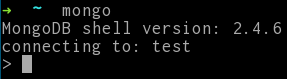
\includegraphics[scale=1]{mongodb_consola} 
    \caption[Consola de MongoDB]{Consola de MongoDB.}
\end{figure}

Al iniciar la consola se conecta autom\'aticamente a la base de datos \textit{\textbf{"test"}}, y apartir de all\'i podemos realizar consultas sobre esa base de datos. La consola es importante para administrar MongoDB, puede parecer desafiante para los que no est\'an acostumbrado a usar herramientas en c\'onsola, pero la gente de 10gen pens\'o en eso y agreg\'o comandos f\'aciles de recordar.

\subsection{Ayuda en la consola interactiva}

Para acceder a la ayuda de MongoDB en la consola, se utiliza el comando \textit{\textbf{help()}}.

\begin{lstlisting}
    > help
	db.help()                    help on db methods
	db.mycoll.help()             help on collection methods
	sh.help()                    sharding helpers
	rs.help()                    replica set helpers
	help admin                   administrative help
	help connect                 connecting to a db help
	help keys                    key shortcuts
	help misc                    misc things to know
	help mr                      mapreduce

	show dbs                     show database names
	show collections             show collections in current database
	show users                   show users in current database
	show profile                 show most recent system.profile entries with time >= 1ms
	show logs                    show the accessible logger names
	show log [name]              prints out the last segment of log in memory, 'global' is default
	use <db_name>                set current database
	db.foo.find()                list objects in collection foo
	db.foo.find( { a : 1 } )     list objects in foo where a == 1
	it                           result of the last line evaluated; use to further iterate
	DBQuery.shellBatchSize = x   set default number of items to display on shell
	exit                         quit the mongo shell
\end{lstlisting}

\section{Conectando a una base de datos}

La conexi\'on a bases de datos desde la consola o a trav\'es de alg\'un lenguaje es muy sencillo; a\'un as\'i en MongoDB NO se crean las bases de datos antes de usarla. En bases de datos relacionales, se debe crear toda una estructura inicial para poder almacenar informaci\'on, al menos se debe tener una base de datos con una tabla, eso en MongoDB no se hace. Para crear una base de datos se debe seleccionar, luego almacenar un documento creando una colecci\'on de documentos.

\subsection{Seleccionando la base de datos}

Antes de seleccionar una base de datos, uno tiene la opci\'on de ver el listado de bases de datos que existen en el sistema, con el comando \textit{\textbf{show dbs}}.

\begin{lstlisting}
    > show dbs
    admin	0.203125GB
    fudcon	0.453125GB
    irianas_server	0.203125GB
    irianas_web	0.203125GB
    local	0.078125GB
    mongoengine	0.203125GB
    mongoenginetest	0.203125GB
    mongoenginetest2	0.203125GB
    mongoenginetest4	0.203125GB
    test_files	0.203125GB
\end{lstlisting}

La salida nos muestra el nombre y el tama\~no de la base de datos, es importante mencionar que MongoDB al crear el primer documento reserva espacio en disco.

Luego de saber la lista de bases de datos existente, debo seleccionar una, no es obligatorio que est\'e en la lista, sencillamente haciendo uso del comando \textit{\textbf{use basededatos}}, se selecciona y podemos trabajar con la base de datos existente u operar para crear una nueva.

\begin{lstlisting}
    > use libromongodb
    switched to db libromongodb
\end{lstlisting}

Para confirmar la selecci\'on de la base de datos "libromongodb" en la sesi\'on, se verifica el valor del objecto \textit{\textbf{"db"}}.

\begin{lstlisting}
    > db
    libromongodb
\end{lstlisting}

\section{Nuestro primer documento}

Lleg\'o la hora de crear una base de datos y una colecci\'on, y eso se har\'a almacenando un documento usando el objeto \textit{\textbf{db}}, previa ejecuci\'on del comando \textit{\textbf{use}}. \textbf{Un documento puede tener en teor\'ia un m\'aximo de hasta 16MB de informaci\'on}. 

Aprovechando el ejemplo del primer cap\'itulo, para por fin almacenarlo en MongoDB y consultarlo. Una de las cosas que hay que tener en cuenta usando la consola interactiva, es usar variables para crear o modificar documentos, de esta manera podemos evitar accidentes con una mala manipulaci\'on directa de la base de datos.

Para almacenar un documento debemos ejecutar el m\'etodo \textit{\textbf{.insert()}} del objeto db, especificando el nombre de la colecci\'on (la colecci\'on se crea de manera din\'amica como la base de datos). Ejemplo:

\begin{lstlisting}
    > documento = {
    ...     _id: 1,
    ...     nombre: "MongoDB",
    ...     url: "http://www.mongodb.org",
    ...     tipo: "Documental"
    ...     }
    {
    	"_id" : 1,
    	"nombre" : "MongoDB",
    	"url" : "http://www.mongodb.org",
    	"tipo" : "Documental"
    }
    > db.nueva_coleccion.insert(documento)
\end{lstlisting}

De esta manera tenemos nuestra primera colecci\'on y nuestro primer documento, para confirmar esto, podemos ejecutar tanto el comando \textit{\textbf{show collections}} como el m\'etodo \textit{\textbf{.find()}}.

\begin{lstlisting}
    > show collections
    nueva_coleccion
    system.indexes
\end{lstlisting}

system.indexes es una colecci\'on que usa MongoDB para almacenar los \'indices de la colecci\'on. Por defecto \textit{\_id} es un \'indice.

\begin{lstlisting}
    > db.nueva_coleccion.find()
    { "_id" : 1, "nombre" : "MongoDB", "url" : "http://www.mongodb.org", "tipo" : "Documental" }
\end{lstlisting}

Con \textit{\textbf{.find()}} se puede comprobar que efectivamente se almacen\'o el documento en la colecci\'on \textit{nueva\_colecci\'on}.
\chapter{CRUD en MongoDB}

\section{?`Qu\'e es CRUD?}

\section{Create}

\section{Read}

\section{Update}

\section{Delete}
\chapter{Operaciones avanzadas en MongoDB}

\section{Operadores relacionales o de comparación}

Los operadores relacionales son símbolos que se usan para comparar dos valores. Si el resultado de la comparación es correcto la expresión considerada es verdadera, en caso contrario es falsa.

\begin{table}[ht] 
\caption{Operadores relacionales}
\centering
\begin{tabular}{c c c c}
\hline\hline
Símbolo & Nombre & Ejemplo & Significado \\ [0.5ex] 
\hline
> & mayor que & A > B & A es mayor que B \\ 
< & menor que & A < B & A es menor que B \\
>= & mayor o igual que & A >= B & A es mayor o igual que B \\
<= & menor o igual que & A <= B & A es menor o igual que B \\ 
== & igual a & A == B & A es igual a B \\ 
!= & distinto a & A != B & A es distinto a B \\ [1ex]
\hline
\end{tabular} 
\label{table:nonlin} 
\end{table}

\subsection{Equivalencia de operadores relaciones en MongoDB}

El motor de base de datos MongoDB permite hacer operaciones sobre colecciones de datos aplicando todos los operadores relaciones de la tabla 4.1, pero con ciertas variaciones.

\begin{table}[ht] 
\caption{Tabla de equivalencias de operadores relacionales}
\centering
\begin{tabular}{c c c c}
\hline\hline
Símbolo & Nombre & Equivalencia \\ [0.5ex] 
\hline
> & mayor que & \bf{\$gt} \\ 
< & menor que & \bf{\$lt} \\
>= & mayor o igual que & \bf{\$gte} \\
<= & menor o igual que & \bf{\$lte} \\
== & igual a & \bf{:} \\ 
!= & distinto a & \bf{\$ne} \\ [1ex]
\hline
\end{tabular} 
\label{table:nonlin} 
\end{table}

La tabla 4.2 muestra claramente las equivalencias de los operadores relacionales \footnote{La equivalencia para "igual a" no existe como tal, cualquier operación donde se especifique el valor exacto luego de dos puntos se considera "igual a"}, pero existen 2 operadores más considerados relacionales en MongoDB los cuales son \textbf{\$in} y \textbf{\$nin}.

\subsection{\$gt (mayor que) | \$gte (mayor o igual que)}

Los operadores \textbf{\$gt (greater)} y \textbf{\$gte (greater or equal)} son operadores que se pueden utilizar para hacer cualquier tipo de operaciones a una coleccion de documentos, el uso es similar tanto si se utiliza en consulta, escritura o borrado de documentos. 

Un ejemplo de busqueda.

\begin{lstlisting}
    > db.personas.find({edad: {$gt: 10}})
    > db.personas.find({edad: {$gte: 10}})
\end{lstlisting}

\subsection{\$lt (menor que) | \$lte (menor o igual que)}

Los operadores \textbf{\$lt (less)} y \textbf{\$lte (less or equal)} son operadores con un uso similar a \$gt y \$gte. 

Un ejemplo de busqueda.

\begin{lstlisting}
    > db.personas.find({edad: {$lt: 10}})
    > db.personas.find({edad: {$lte: 10}})
\end{lstlisting}

\subsection{Operador de igualdad y desigualdad}

El operador de igualdad en MongoDB no se ve reflejado en simbolos como los operadores de desigualdad, sencillamente son los dos puntos seguidos al valor de la igualdad.

\begin{lstlisting}
    > db.personas.find({edad: 10})
\end{lstlisting}

Este ejemplo consulta todos los documentos que tengan un campo edad igual a 10.

En caso contrario, la desigualdad si tiene una equivalencia \$ne, que significa \textbf{not equal}, y su uso es similar a los otros operadores de mayor que, menor que, mayor igual que y menor o igual que.

\subsection{\$in (Existe en) | \$nin (No existe en)}

Existen dos operadores relacionales adicionales \textbf{\$in (exist in)} y \textbf{\$nin (do not exist in)}, que serían similar al cuantificador existencial en Matemáticas que se denota con $\exists$. \$in busca todos los documentos que coicidan con al menos uno de los valores contenido en el array de valores para la busqueda, y \$nin busca todos los documentos que no tengan campos que coincidan con los valores del array.

Ejemplo:

\begin{lstlisting}
    > db.personas.find({edad: {$in: [9, 10]}})
\end{lstlisting}

En este ejemplo MongoDB busca todos los documentos que tengan un campo edad con valor 9, 10 o ambos.

\begin{lstlisting}
    > db.personas.find({edad: {$nin: [9, 10]}})
\end{lstlisting}

En este otro ejemplo MongoDB busca todos los documentos en el cual el campo edad no coincidan con los valores 9, 10 o ambos.

\section{Operadores logicos}


\chapter{MongoDB en Python y NodeJS}


\backmatter
\include{glosario} 

\printindex
\end{document}